\documentclass{beamer}
\usetheme{Boadilla}
\usepackage{graphicx}
\usepackage{color}
\graphicspath{ {./images/} }
\usepackage{float}
\usepackage[caption = false]{subfig}
\begin{document}

\title{Mandatory 2}
\subtitle{IN5450}
\author{Espen Lønes}
\institute{}
\date{\today}

\begin{frame}
	\titlepage
\end{frame}

\begin{frame}
	\frametitle{Power estimation from classical and adaptive beamforming}
    \begin{itemize}
    \item R
    \item Classical / DAS
    \item Capon's / MV
    \item Eigenvalues / vectors (signal+noise / noise spaces)
    \item Eigenvalue
    \item MUSIC
    \end{itemize}
\end{frame}

\begin{frame}
	\frametitle{The problem}
	\begin{itemize}
		\item 10 element ULA array, with $\lambda / 2$ spacing.
		\item Two incoherent signals at -10 and 0 degrees, with added spatially white noise.
		\item SNR is 0 for both sources.
		\item 100 time samples per element.
		\item Data generated from (fixed) 'generate\_data.m'
	\end{itemize}
\end{frame}

\begin{frame}
	\frametitle{Spatial correlation matrix R}
	\begin{figure}
		\centering
    	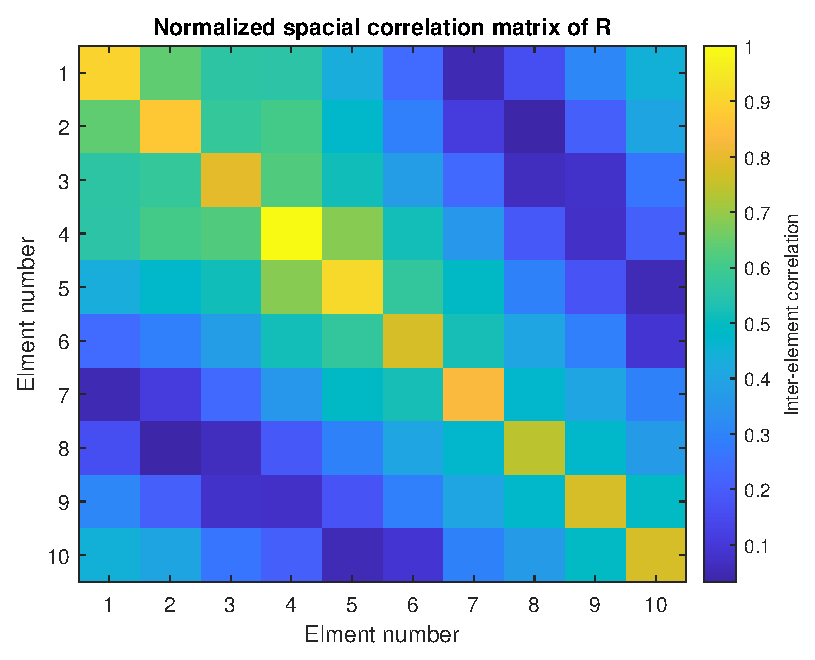
\includegraphics[scale=0.4]{R.eps}\\
    	\caption{Caption}	
	\end{figure}
    $R = x \cdot x^H$\\
    Correlation is a statistical relationship between two variables.\\
\end{frame}

\begin{frame}
	\begin{figure}
    	\frametitle{Classical / DAS beamformer}
		\centering
    	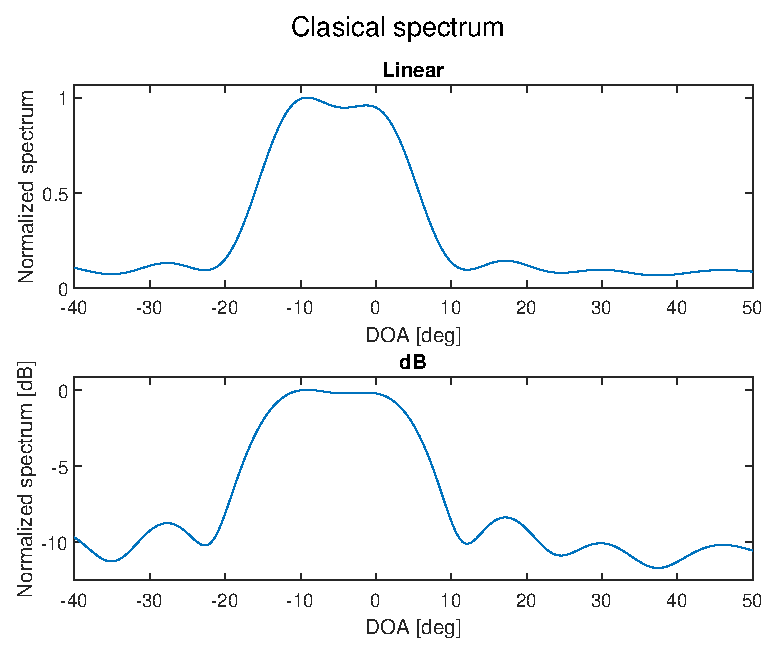
\includegraphics[scale=0.4]{Classical.eps}\\	
	\end{figure}
    $P(w) = w^H R w$\\
    $max_w\ E(w^H R w) = max_w\ w^H (E(R))w \rightarrow w_{bf} = \frac{a(\theta)}					 		{\sqrt{a(\theta)^H a(\theta)}};\ \ |w|=1$\\
    $P_{DAS}(\theta) = \frac{a^H R a}{a^H a}$\\
    $a_j = exp(j*-kd*sin(\theta*pi/180) * (j-1));\ \  j=1, ... ,10$
 \end{frame}

\begin{frame}
	\begin{figure}
    	\frametitle{Capon's / Minimum variance beamformer}
		\centering
    	\includegraphics[scale=0.4]{Capon.eps}\\
	\end{figure}
    $P(w) = w^H R w$\\
    $min_w\ E(w^H R w);\ \ w^H a(\theta)=1$\\
    $w_{CAP} = \frac{R^{-1} a}{a^H R^{-1} a}$\\
    \ \\
    $P_{MV}(\theta) = \frac{1}{a^H R^{-1} a}$\\
\end{frame}

\begin{frame}
	$R = U \Lambda U^H$
	\begin{figure}
    	\frametitle{Eigenvalues of R}
		\centering
    	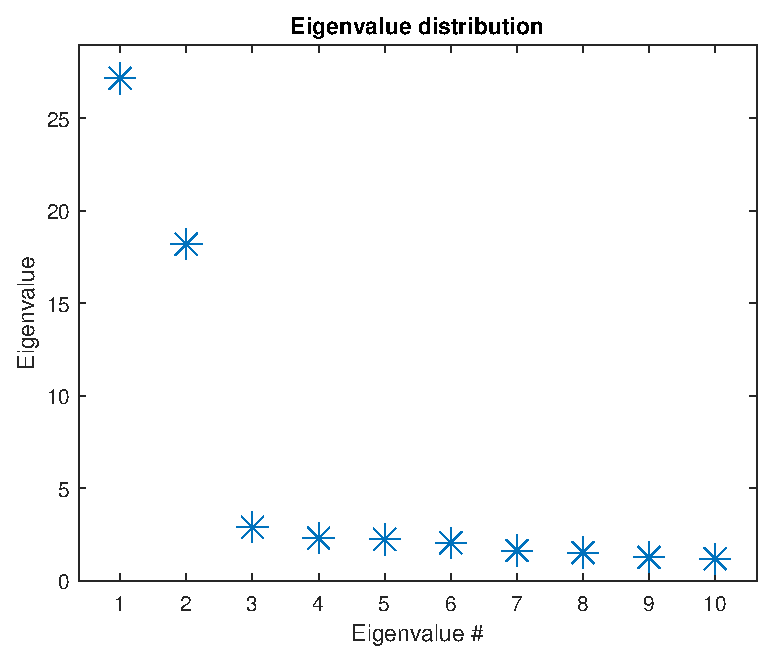
\includegraphics[scale=0.4]{Eigenvalues.eps}\\
	\end{figure}
    Based on the signal and noise model we know that the eigenvectors corresponding to the 		 	largest eigenvalues span the signal+noise space. While the smallest span the noise space.\\
 	Largest != signal. But signal vectors are linear combinations.
\end{frame}

\begin{frame}
	\begin{figure}
    	\frametitle{MUSIC beamformer with 2 sources}
		\centering
    	\includegraphics[scale=0.4]{Music.eps}\\
	\end{figure}
    $R = U_s \Lambda_s U^H_s + U_n \Lambda_n U^H_n$\\
    $U^H_n a(\theta) = 0,\ \ \theta \in (1,...,M),$\ \ (But we have estimates)\\
    2 Sources $\rightarrow$ We use 8 of 10 eigenvectors.\\
    $\Pi = U_n U^H_n\ \ \text{Orthogonal projector onto noise subspace}$\\
    $P_{MUSIC} = \frac{a^H a}{a^H \Pi a}$\\
\end{frame}

\begin{frame}
	Again we use 8 of 10 eigenvectors.
	\begin{figure}
    	\frametitle{Eigenvector beamformer with 2 sources}
		\centering
    	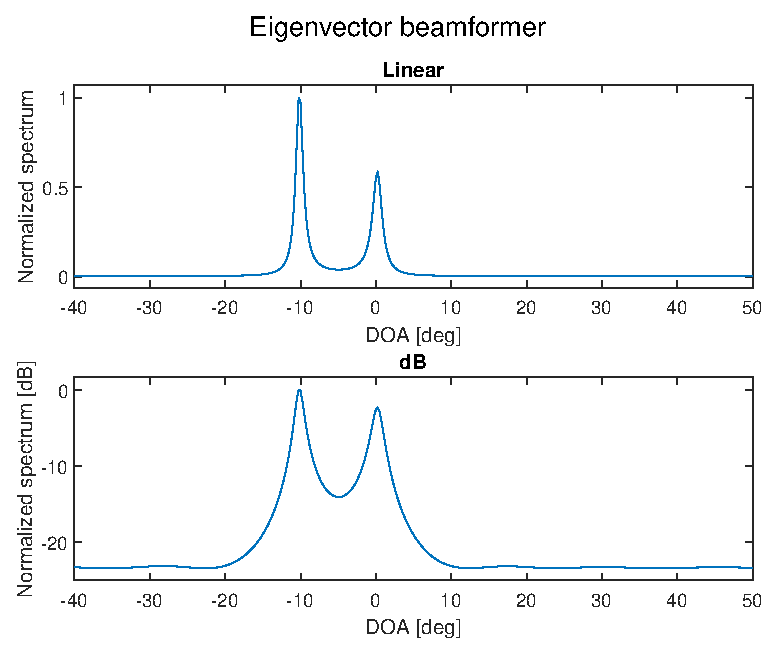
\includegraphics[scale=0.4]{EV.eps}\\	
	\end{figure}
    Similar to MUSIC and uses noise space eigenvalue matrix as well\\
    $P_{EV} = \frac{a^H a}{a^H U_n \Lambda_n^{-1} U^H_n a}$\\
    Diagonal elements of $\Lambda_n^{-1}$\\ 
    $0.3469, 0.4354, 0.4481, 0.4883, 0.6131, 0.6589, 0.7917, 0.8437$
\end{frame}

\begin{frame}
	0 Sources $\rightarrow$ We use 10 of 10 eigenvectors.\\
	\begin{figure}
    	\frametitle{Assuming 0 sources}
		\subfloat{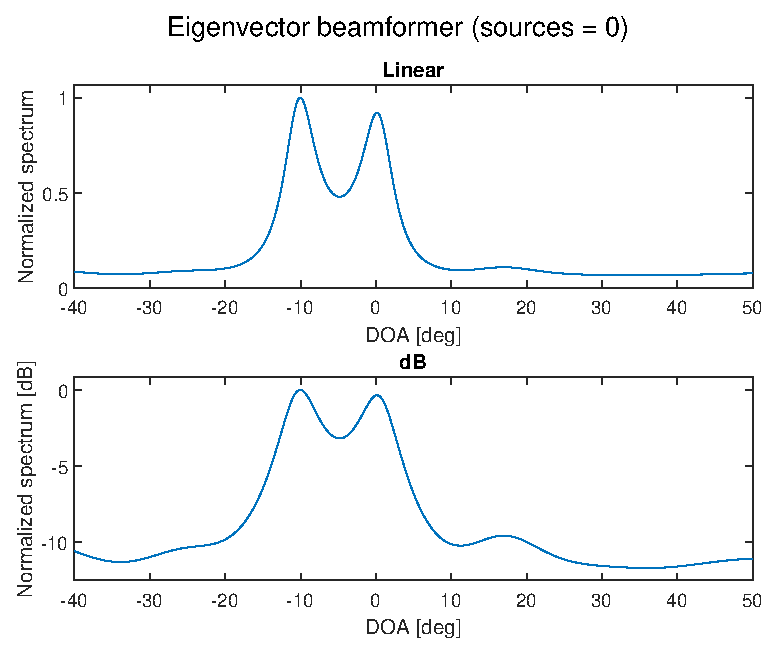
\includegraphics[width = 2in]{images/EV_0_sources.eps}}
		\subfloat{\includegraphics[width = 2in]{images/Music_0_sources.eps}} 	
    	\label{some example}
	\end{figure}
    For 0 sources, $U_n \Lambda_n^{-1} U^H_n = R^{-1}$. So it is like the MV beamformer.\\
    MUSIC whitens noise, 0 sources corresponds to only noise. 
\end{frame}

\begin{frame}
	\begin{figure}
    	\frametitle{Assuming 1 source}
		\subfloat{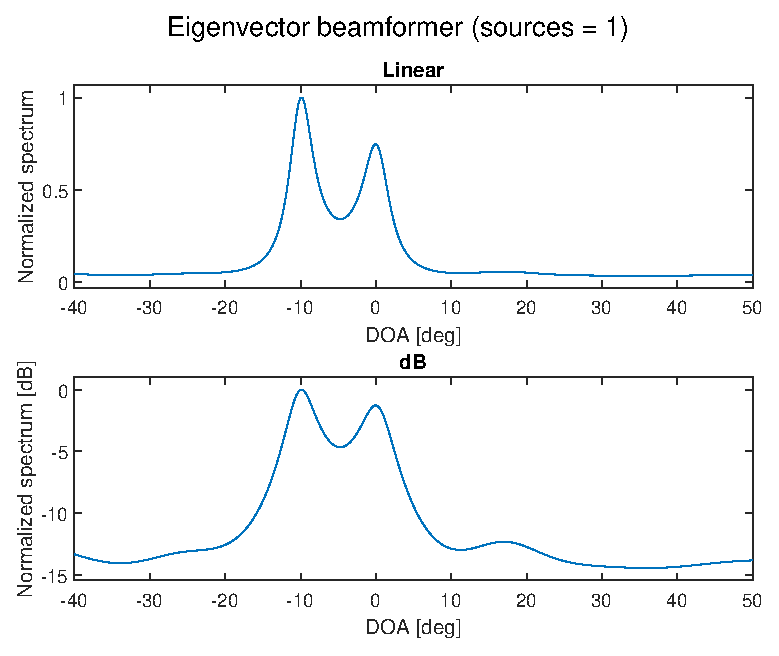
\includegraphics[width = 2in]{images/EV_1_sources.eps}}
		\subfloat{\includegraphics[width = 2in]{images/Music_1_sources.eps}} 
    	\label{some example}
	\end{figure}
    
\end{frame}

\begin{frame}
	\begin{figure}
    	\frametitle{Assuming 3 sources}
		\subfloat{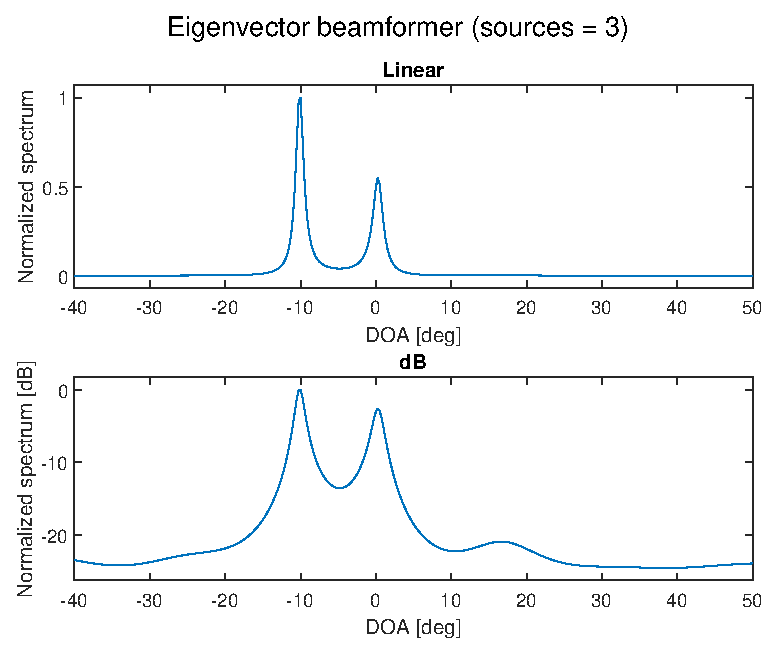
\includegraphics[width = 2in]{images/EV_3_sources.eps}}
		\subfloat{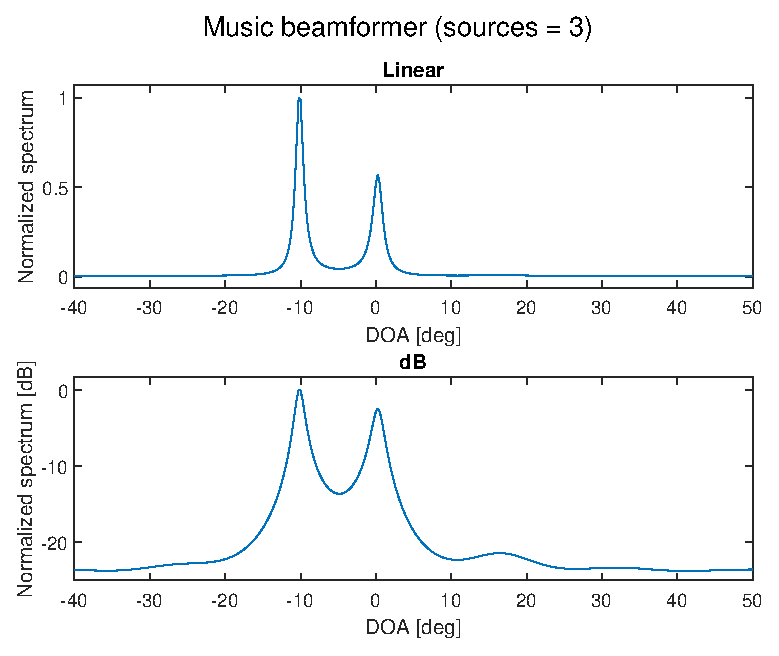
\includegraphics[width = 2in]{images/Music_3_sources.eps}} 	
    	\label{some example}
	\end{figure}
    
\end{frame}

\begin{frame}
	\frametitle{References}
	\begin{itemize}
		\item H. Krim, M. Viberg, Two decades of array signal processing research 
		– The parametric approach, IEEE Signal Processing Magazine,\\ pp. 67–94, July 1996, 
		\url{http://dx.doi.org/10.1109/79.526899}
	\end{itemize}
\end{frame}

\end{document}